\section{Scintillation Detectors}
\subsection{General Remarks}
\begin{itemize}
    \item Preferred in applications where high efficiency is more important than energy resolution (e.g., medical imaging, Compton suppression).
    \item Available as solids, liquids, and gases; useful in detecting all types of ionizing radiation including fast (organic with H) and slow neutrons (Li, B, Gd). 
\end{itemize}

\subsection{Scintillation Detection Principles and Counters}
\subsubsection{Requirements of Scintillators}
\begin{itemize}
    \item High light/ scintillation/ fluorescence yield
    \item Linear conversion of $\Delta E$ to scintillation photons
    \item Transparent to scintillation photons to minimize self-absorption
    \item Short decay time of fluorescence (ps$\sim$ns) for generation of fast pulses
    \item Good optical quality with sufficient size
    \item Index of refraction $n\sim1.5$ (glass) for efficient coupling to readout device (PMT or other light sensors)
    \item Fluorescence wavelength matches spectral response of readout device
\end{itemize}

\subsubsection{Types of Scintillators}
\begin{enumerate}
    \item Organic
    \begin{itemize}
        \item Liquids, crystals, and plastics
        \item Low Z and low density
        \item Low and \emph{non-linear} light output
        \item Fast decay times
        \item High H content allows fast neutron detection
        \item Pulse-shape discrimination between various particles
    \end{itemize}
    \item Inorganic
    \begin{itemize}
        \item Crystals such as alkali-halide (M$^+$X$^-$)
        \item High Z and high density
        \item High and (relatively) linear light output
        \item Slower decay times
    \end{itemize}
\end{enumerate}
\begin{figure}[ht]
    \centering
    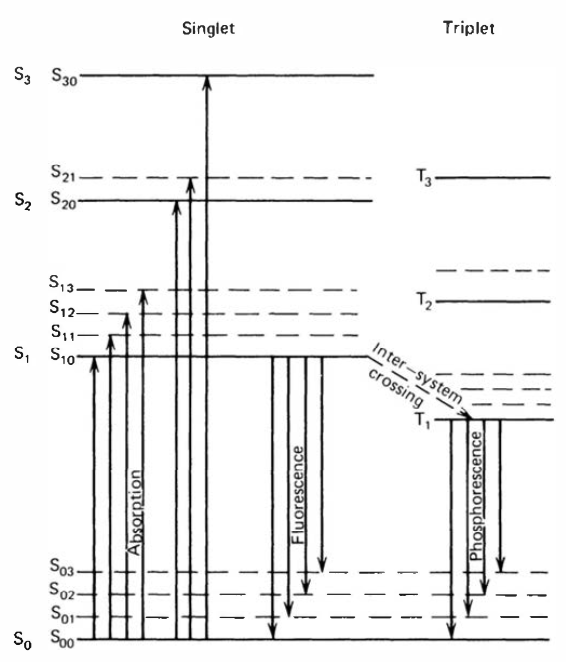
\includegraphics[width=0.4\textwidth]{images/organic_scintillator_energy_level.png}
    \caption{Energy levels of an organic molecule with the $\pi$-electron structure.}
    \label{fig:organic_scintillator_energy_level}
\end{figure}
\subsubsection{Organic Scintillators}
\begin{itemize}
    \item Fluorescence arises from transitions in the energy level structure of a single molecule, independent of physical state (solid, liquid, gas).
    \item The ground state of electrons in the $S_{00}$ singlet state (second index denotes vibration states), and interactions populate higher $S$ states, followed by rapid radiation-less de-excitations into the $S_{10}$ state. Prompt fluorescence is emitted by $S_{10}$ to $S_{0x}$ transitions. See figure~\ref{fig:organic_scintillator_energy_level}.
    \item Some singlet states decay into triplet ($T$) states with much longer lifetimes.
    \item As shown in figure~\ref{fig:organic_scintillator_energy_level}, the $T_1$ to $S_0$ state can be via a delayed light emission characterized as phosphorescence. 
    \item Since the $T_1$ state lies below the $S_0$ state, molecules in the $T_1$ state can be thermally excited back to the $S_1$ state before decaying through normal fluorescence. This is the origin of the delayed fluorescence sometimes observed for organics. 
    \begin{itemize}
        \item The light output is therefore described by a fast component and a slow component:
        \item[] $N=A\exp\left(-\frac{t}{\tau_f}\right)+B\exp\left(-\frac{t}{\tau_s}\right)$
    \end{itemize}
    \item The fact that the fraction of light that appears in the slow component depends on the nature of the exciting particles allows for pulse shape discrimination. Figure~\ref{fig:organic_scintillator_psd} shows the differences in the slow component of various particles with different ionizing density. 
    \begin{figure}[ht]
        \centering
        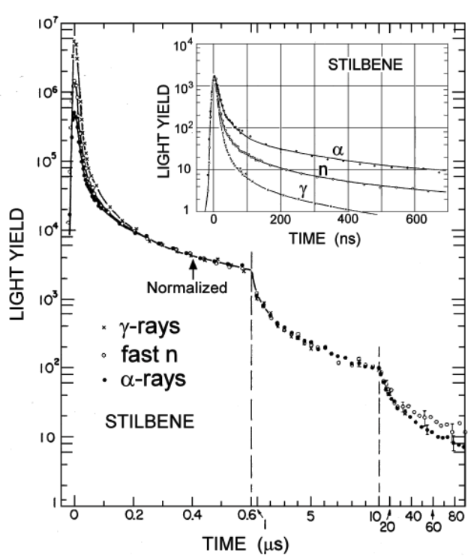
\includegraphics[width=0.4\textwidth]{images/organic_scintillator_psd.png}
        \caption{Pulse-shape discrimination.}
        \label{fig:organic_scintillator_psd}
    \end{figure}
    \item Since energies of the fluorescence transitions (downward arrows in figure~\ref{fig:organic_scintillator_energy_level}) are lower than the photon energies that would be strongly absorbed in the material (upward arrows), there is very little overlap between the optical absorption and emission spectra (Stokes shift). Organic scintillators can therefore be transparent to their own fluorescence emission.
    \item Scintillation efficiency is defined as the fraction of all incident particle energy that is converted into visible light. While we wish to maximize this efficiency, alternate de-excitation modes exist, in which the excitation is degraded mainly into heat. These radiation-less de-excitations are grouped under the term \emph{quenching}.
    \item Linearity between light yield and initial energy builds on the independence of the scintillation efficiency on energy. For organic scintillators, the response to electrons above 125 keV is linear, but for heavy charged particles (proton, alpha), the light yield is not only lower but also non-linear to higher energies, as shown in figure~\ref{fig:organic_scintillator_proton_nonlinear}. 

    \begin{figure}[ht]
        \centering
        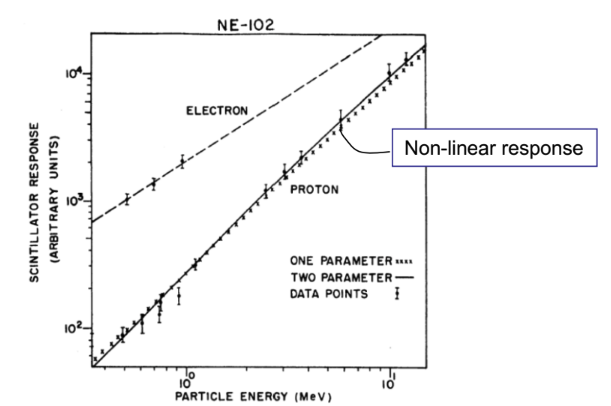
\includegraphics[width=0.5\textwidth]{images/organic_scintillator_proton_nonlinear.png}
        \caption{Non-linearity of light yield in organic scintillators.}
        \label{fig:organic_scintillator_proton_nonlinear}
    \end{figure}
\end{itemize}

\subsubsection{Inorganic Scintillators}
\begin{figure}[ht]
    \centering
    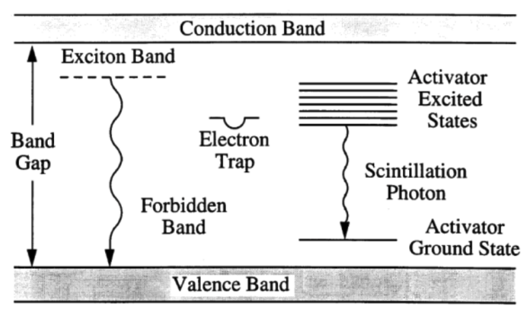
\includegraphics[width=0.4\textwidth]{images/inorganic_scintillator_band_structure.png}
    \caption{Band structure or an activated crystalline (inorganic) scintillator.}
    \label{fig:inorganic_scintillator_band_structure}
\end{figure}
\begin{itemize}
    \item As in semiconductor detectors, the primary radiation creates electron-hole pairs (excitons) in the crystal lattice, which can migrate independently. However, in this case, recombination and de-excitation through light emission is the goal.
    \item Since, as shown in figure~\ref{fig:inorganic_scintillator_band_structure}, there is a forbidden band in between the conduction and valence bands, to enhance the probability of visible photon emission during the de-excitation process, \emph{activators} are added to create energy states within the gorbidden gap through which electrons can de-excite back into the valence band. This transition gives rise to a visible photon; the de-excitation sites are termed ``luminescence centers'' or ``recombination centers''. See figure~\ref{fig:inorganic_scintillator_activator_concentration} for the impact of activator concentration. 
    \item Since the de-excitation goes through activator states with smaller energy differences than the band gap, there is no self-absorption of photons in the material. 
    \item Competitions with the aforementioned process can occur. An excited electron may need an extra increment of energy (thermal excitation) to reach a higher-lying state from which de-excitation to the ground state is possible, and lead to a slow component of light (phosphorescence). An electron can also de-excite via radiation-less transitions (quenching). 
\end{itemize}
\begin{figure}[ht]
    \centering
    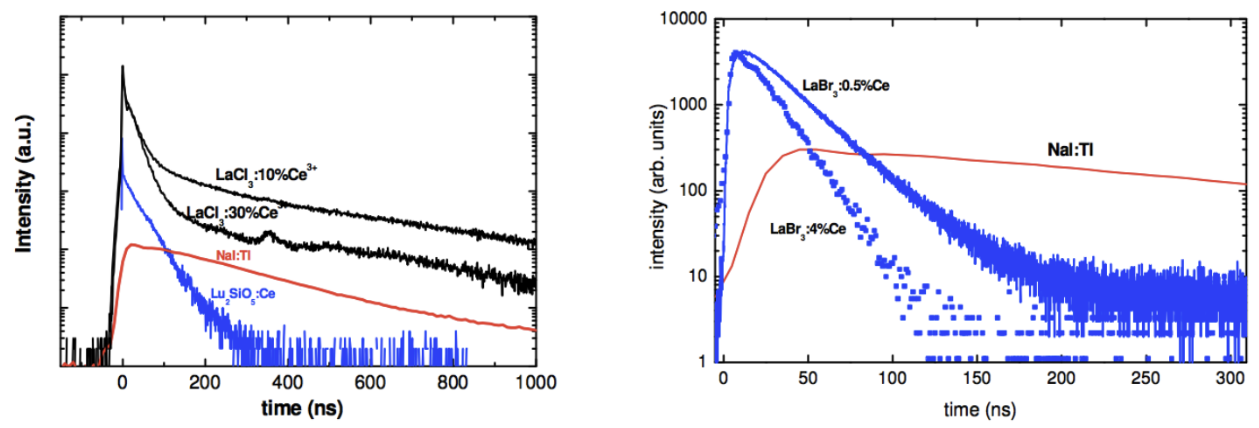
\includegraphics[width=0.8\textwidth]{images/inorganic_scintillator_activator_concentration.png}
    \caption{Impact of activator (Ce) concentration on inorganic scintillators (NaI(Tl), LaCl$_3$ and LaBr$_3$). Note that NaBr$_3$(Ce) scintillators have very good general performance, with high energy resolution (2.5\% at 662 keV) and small rate of change of light output with temperature.}
    \label{fig:inorganic_scintillator_activator_concentration}
\end{figure}
\subsubsection{Comparison of Scintillators}
\begin{center}
\begin{tabular}{|c|c|c|}
    \hline
     & Inorganic & Organic \\
    \hline
    Mechanism & Exciton (electron-hole) recombination & De-excitation of molecular $\pi$-electrons \\
    \hline
    Efficiency & Wide range: 0.001 (PWO) $\sim$ 0.1 (NaI(Tl)) & Narrow range: 0.02 $\sim$ 0.04 \\
    \hline
    Track quenching & Small & Large \\
    \hline
    Time constant & Slow ($\mu$s) & Fast (10's of ns) \\
    \hline
    Density & Generally high & Always low\\
    \hline
    $\gamma$-ray detection & Important & Nearly insensitive \\
    \hline
    PSD & Possible in some cases & Fast/ slow for $\gamma$/ n\\
    \hline
\end{tabular}
\end{center}

\subsection{Scintillator Readout}
\subsubsection{Photomultiplier Tubes}
\begin{figure}[ht]
    \centering
    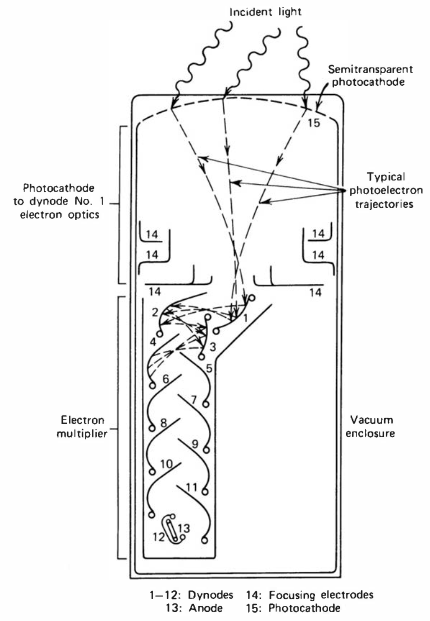
\includegraphics[width=0.4\textwidth]{images/PMT_config.png}
    \caption{Simplified structure of a PMT.}
    \label{fig:PMT_config}
\end{figure}
\begin{itemize}
    \item The PMT converts scintillation light electrical signals.
    \item An outer (glass) envelope sustains vacuum condition inside the tube. A photocathode is coupled to an electron multiplier structure. 
    \item The main three components are:
    \begin{enumerate}
        \item Photocathode:\\
        Photocathodes should have
        \begin{itemize}
            \item High quantum efficiency (QE): 
            \begin{itemize}
                \item[] $\text{QE}=\text{\# photoelectrons emitted}/\text{\# incident photons}$
            \end{itemize}
            \item Low electron negativity (the potential barrier between the material's conduction band and the vacuum)
            \item Low work function (the potential barrier at the interface of the vacuum and the material's valence band)
            \item Thin and uniform layer ($\sim$30 nm) to allow photoelectrons to escape
        \end{itemize}
        \item Dynodes:
        \begin{itemize}
            \item Similar process as in the photocathode, but with electrons as incident particles. 
            \item Electrons are accelerated between dynodes ($\Delta$V$\sim$100V), penerates into the material, and release secondary electrons. 
            \item The gain (multiplication factor) of a single dynode is given as:
            \begin{itemize}
                \item[] $\delta=\text{\# secondary electrons emitted}/\text{\# primary incident electrons}$
            \end{itemize}
            \item Typical gain $\delta\sim5$, and with $N=$3$\sim$10 dynodes, the total gain of the tube $M=\delta^N$\\
            Slight changes in $\delta$ can lead to large charges in $M$.
            \item $\delta$ depends on the primary electron energy.
        \end{itemize}
        \item Anode
    \end{enumerate}
\end{itemize}

\subsubsection{Other Multiplication Devices}
\begin{itemize}
    \item Microchannel plates (MCP): 
    \begin{itemize}
        \item Continuous multiplication
        \item Good timing properties
        \item Allows position sensitive detection of photons
    \end{itemize}
    \item Gaseous electron multiplier (GEM):
    \begin{itemize}
        \item Derivatives of gas-filled proportional counters
        \item Allows position sensitive detection of photons
    \end{itemize}
    \item Photodiodes:
    \begin{itemize}
        \item Can be preferred in certain applications over PMTs with the advantages of: higher quantum efficiency (potentially better energy resolution), lower power consumption, compact size, insensitive to magnetic fields, comparable time response (useful in coincidence applciations).
        \item Si-based photodiodes:\\
        Very similar to Si semiconductor detectors, worse energy resolution than PMTs.
        \item Avalanche photodiodes (APD):\\
        Electron multiplication/ avalanche due to high electric field; can have good energy resolution with proper (temperature, voltage) stabilization schemes. 
        \item SiPM (silicon photomultiplier):\\
        An array of small APDs operated in Geiger mode (gain of $10^6$ with single photon sensitivity); the sum of counts from each element reflects the total number of photons and incident energy.
    \end{itemize}
\end{itemize}

\subsection{Scintillator Performance}
\subsubsection{Statistics and Energy Resolution}
The statistics of scintillation detectors are affected by various factors in the following steps:
\begin{enumerate}
    \item Absorption of incident particle in the scintillator
    \begin{itemize}
        \item[] Example: 511 keV in NaI(Tl)
    \end{itemize}
    \item Population of excited states (time constant)
    \item Decay of states (time constant, absorption, reflection)
    \begin{itemize}
        \item[] 25000 photons in the crystal
    \end{itemize}
    \item Absorption in the photocathode (transmission in glass, quantum efficiency)
    \begin{itemize}
        \item[] 3000 electrons at the first dynode
    \end{itemize}
    \item Multiplication of photoelectrons
    \begin{itemize}
        \item[] 3$\times$10$^9$ electrons at the anode
    \end{itemize}
\end{enumerate}
The uncertainty is largely determined by the number of electrons at the first dynode:\\
$\Delta E/E=2.355\sqrt{1/3000}=0.043$

\subsubsection{Comparison of Scintillation and HPGe Detectors}
\begin{itemize}
    \item Scintillators have Fano factor $\sim$1, so the statistical limit of energy resolution is
    \begin{itemize}
        \item[] $\text{FWHM}=2.355\sqrt{E\times E_I}$
        \item[] With $E=662$ keV and $E_I=0.23$ keV,
        \item[] $\text{FWHM}=29$ keV ($4.4$\%)
    \end{itemize}
    \item Additional contributions to the FWHM include:
    \begin{itemize}
        \item Uncertainty in the electron multiplication process
        \item Non-linearity in light yield
    \end{itemize}
    \item The best FWHM at 662 keV is $\sim$6\% for NaI(Tl) detectors; HPGe detectors have resolution $\sim$0.2\% (a factor of 30 better). See figure~\ref{fig:HPGe_scintillator_comparison} for comparison of spectra. 
\end{itemize}
\begin{figure}[ht]
    \centering
    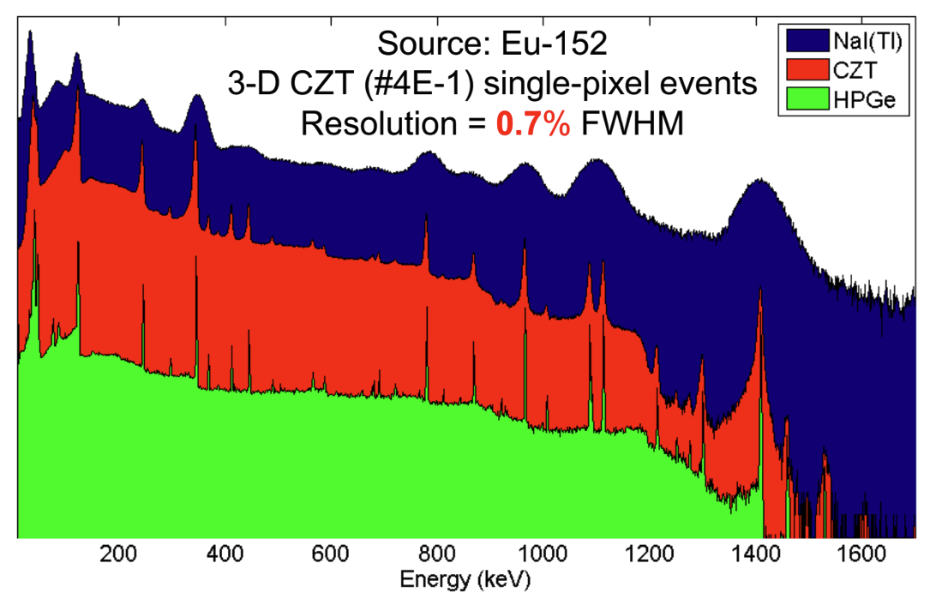
\includegraphics[width=0.4\textwidth]{images/HPGe_scintillator_comparison.png}
    \caption{Energy resolution comparison of HPGe and NaI(Tl) detectors. Note that the (pixelated) CZT detector is another solid state detector.}
    \label{fig:HPGe_scintillator_comparison}
\end{figure}
\subsubsection{Limitations of Scintillators}
Achievable energy resolution in scintillation detectors is limited by the non-proportionality of light-yield, as shown in figure~\ref{fig:scintillator_nonlinearity}. 
\begin{itemize}
    \item Since a variable amount of energy is deposited in each interaction, and that the interactions cannot be resolved, the non-proportionality in light yield inherently limits the energy resolution.
    \item The non-proportionality increases the variance in the number of information carriers (photons), hence increases the Fano factor.
    \item The Fano factor of scintillator is typically $\sim$1, depending on material-specific quenching and amplication processes.
\end{itemize}
\begin{figure}[ht]
    \centering
    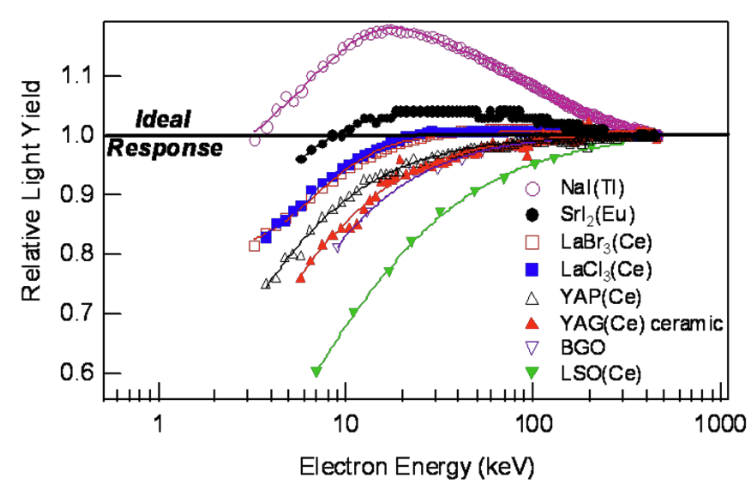
\includegraphics[width=0.5\textwidth]{images/scintillator_nonlinearity.png}
    \caption{Dependence of light yield on electron energy, characterized by SLYNCI (scintillation light yield non-proportionality characterization instrument).}
    \label{fig:scintillator_nonlinearity}
\end{figure}